\documentclass[10pt,a4paper,openany,twoside,prof]{book}

\usepackage{layout_cours}
\usepackage{hyperref}

\setlist{leftmargin=5mm}

\begin{document}
	\chapnumber{2} % numéro du chapitre
	\titre{Géométrie vectorielle} % titre du chapitre
	\classe{Seconde} % classe
	\entetegal

	% Debut du texte
	% **************
	\vspace{-7mm}
	\paragraph*{Objectif du chapitre:}
	\begin{itemize}  
		\vspace{-2mm}
		\setlength\itemsep{-1mm}
		\item Utiliser les vecteurs pour résoudre des problèmes de géométrie
		\item Comprendre le vocabulaire associé au vecteurs : colinéarité, représentant, translation
	\end{itemize}
	\vspace{-7mm}

\section{Translation}

\begin{defi}{Translation}{}
Une \bf{translation} déplace tous les points d'un objet géométrique de la même distance, selon la même direction et dans le même sens.

\begin{center}
	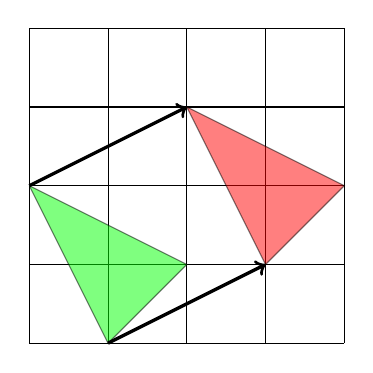
\begin{tikzpicture}
		\draw (-2,-2) grid (2,2);
		\draw[fill=green, opacity=0.5] (-2, 0) -- (-1, -2) -- (0,-1) -- (-2, 0);
		\draw[fill=red, opacity=0.5] (0, 1) -- (1, -1) -- (2,0) -- (0, 1);
		\draw[->,very thick] (-2, 0) --(0, 1);
		\draw[->,very thick] (-1, -2)  --( 1, -1) ;
	\end{tikzpicture}
\end{center}

\end{defi}

\begin{defi}{Vecteur}{}
	A chaque translation, on associe un vecteur noté $\vecu$. Un vecteur se définit donc avec 
	
	\begin{itemize}
		\item 
		une norme (distance de la translation) noté $\norm{\vecu}$
		\item une direction (axe de la translation)
		\item un sens
	\end{itemize}

	On distingue le vecteur nul $\vec{0}$ qui a une norme nulle et n'a pas de direction ni de sens. Il correspond à un déplacement nul.
\end{defi}

\begin{notation}{Vecteur $\vec{AB}$}{}
	Le vecteur associé à la translation qui transforme le point A en le point B est noté $\vec{AB}$. On représente le vecteur par une flèche.
\end{notation}


\begin{prop}{Egalité de vecteurs}{}
	On dispose de trois manières de tester que deux vecteurs sont égaux : 
	\begin{itemize}
		\item Par définition, deux vecteurs $\vec{AB}$ et $\vec{CD}$ sont égaux s'ils décrivent la même translation.
		\item De façon équivalente, deux vecteurs sont égaux s'ils sont tous les deux nuls; ou s'ils ont même norme, même direction et même sens.
		\item Deux vecteurs $\vec{AB}$ et $\vec{CD}$  sont égaux si et seulement si le quadrilatère ABDC est un parallélogramme (éventuellement aplati).
	\end{itemize}
	
	On dit alors qu'ils sont des \bf{représentants} du même vecteur que l'on peut nommer avec une seule lettre, par exemple $\vecu$. On note $\vec{AB} = \vec{CD}$. Il y a une infinité de \bf{représentants} du même vecteur $\vecu$.

	\begin{minipage}{0.4 \linewidth}
		\begin{center}
			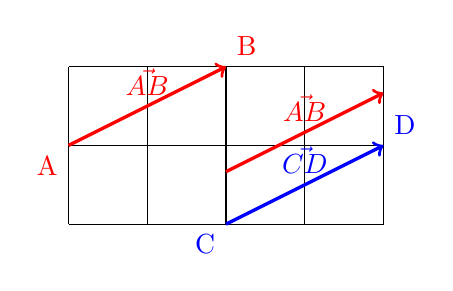
\begin{tikzpicture}
				\draw (-1,-1) grid (3,1);
				\draw[->,very thick, red] (-1, 0) node[below left] {A} -- node[above] {$\vec{AB}$} (1, 1) node[above right] {B};
				\draw[->,very thick, blue] (1, -1) node[below left] {C} -- node[above] {$\vec{CD}$} (3, 0) node[above right] {D};
				\draw[->,very thick, red] (1, -1/3) -- node[above] {$\vec{AB}$} (3, 2/3);

			\end{tikzpicture}
		\end{center}
	\end{minipage}
	\begin{minipage}{0.4 \linewidth}
	\begin{center}
		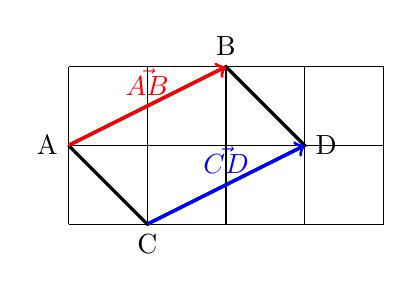
\begin{tikzpicture}
			\draw (-1,-1) grid (3,1);
			\draw[very thick] (-1, 0) node[left] {A} -- (1, 1) node[above] {B} -- (2,0) node[right] {D} -- (0,-1) node[below] {C} -- (-1, 0);
			
			\draw[->,very thick, red] (-1, 0) -- node[above] {$\vec{AB}$} (1, 1);
			\draw[->,very thick, blue] (0,-1) -- node[above] {$\vec{CD}$} (2,0);
		\end{tikzpicture}
	\end{center}
	\end{minipage}
\end{prop}

\begin{defi}{Opposé d'un vecteur}{}
		Le vecteur $\vec{BA}$ est l'opposé du vecteur $\vec{AB}$. Il a même norme, même direction et un sens opposé. Il réalise la translation inverse.
		
		\begin{center}
			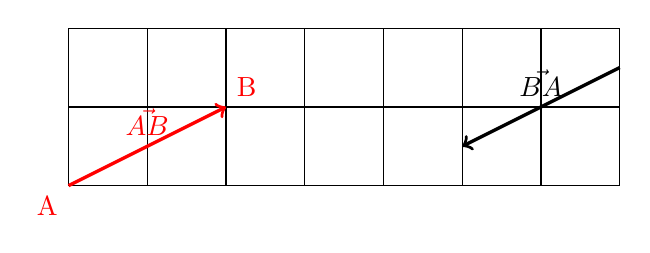
\begin{tikzpicture}
				\draw (-1,0) grid (6,2);
				\draw[->,very thick, red] (-1, 0) node[below left] {A} -- node[above] {$\vec{AB}$} (1, 1) node[above right] {B};
				\draw[->,very thick] (6, 3/2) -- node[above] {$\vec{BA}$} (4, 1/2);
			\end{tikzpicture}
		\end{center}
	
\end{defi}

\section{Opérations sur les vecteurs}

\begin{defi}{Somme de vecteurs}{}
	Si on applique la translation associée à  $\vecu$, puis la translation associée à $\vecv$, on obtient une nouvelle translation. Le vecteur de cette nouvelle translation est la \bf{somme des vecteurs} $\vecu+\vecv$. 

	\begin{center}
		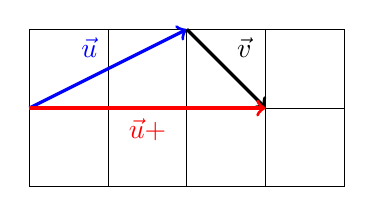
\begin{tikzpicture}
			\draw (-1,-1) grid (3,1);
			\draw[->,very thick, blue] (-1, 0) -- node[above left] {$\vec{u}$} (1, 1);
			\draw[->,very thick] (1, 1)-- node[above right] {$\vec{v}$} (2,0);
			\draw[->,very thick, red] (-1, 0) -- node[below] {$\vec{u}+\vecv$} (2,0);
		\end{tikzpicture}
	\end{center}

\end{defi}

\begin{prop}{}{}
	Il n'y a pas d'ordre dans la somme : $\vecu+\vecv = \vecv+\vecu$. On dit que la somme est commutative
\end{prop}

\begin{theo}{Relation de Chasles}{}
	Soient trois points A, B, C du plan. On a $\vec{AB}+\vec{BC}=\vec{AC}$.
		\begin{center}
		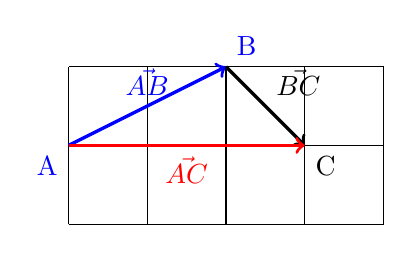
\begin{tikzpicture}
			\draw (-1,-1) grid (3,1);
			\draw[->,very thick, blue] (-1, 0) node[below left] {A} -- node[above] {$\vec{AB}$} (1, 1) node[above right] {B};
			\draw[->,very thick] (1, 1)-- node[above right] {$\vec{BC}$} (2,0) node[below right] {C};
			\draw[->,very thick, red] (-1, 0) -- node[below] {$\vec{AC}$} (2,0);
		\end{tikzpicture}
	\end{center}
\end{theo}

\begin{prop}{Somme $\vec{AB}+\vec{AC}$}{}
	Soit A, B, C des points distincts. Soit D tel que ABCD soit un parallélogramme. On a alors  $\vec{AB}+\vec{AC}=\vec{AD}$.
\end{prop}

\begin{dem}{}{}
	Puisque ABCD est un parallélogramme, les côtés $[AC]$ et $[BD]$ sont parallèle et de même longueur. Donc $\vec{AC} = \vec{BD}$.

	On calcule donc : $\vec{AB}+\vec{AC} = \vec{AB}+\vec{BD} = \vec{AD}$ en utilisant la relation de Chasles.

	\begin{center}
		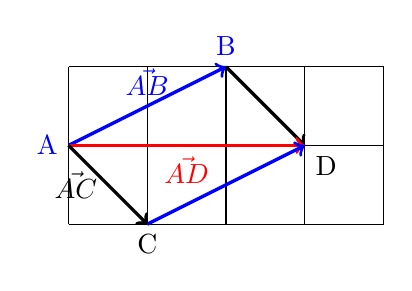
\begin{tikzpicture}
			\draw (-1,-1) grid (3,1);
			\draw[->,very thick, blue] (-1, 0) node[left] {A} -- node[above] {$\vec{AB}$} (1, 1) node[above] {B};
			\draw[->,very thick] (1, 1)-- (2,0) node[below right] {D};
			\draw[->,very thick, red] (-1, 0) -- node[below] {$\vec{AD}$} (2,0);
			\draw[->,very thick, blue] (0,-1) -- (2,0);
			\draw[->,very thick] (-1, 0) -- node[left] {$\vec{AC}$} (0,-1) node[below] {C};
		\end{tikzpicture}
	\end{center}
\end{dem}

\begin{notation}{}{}
	Soit $x\in\R$ un réel. On note $|x|$ la \bf{valeur absolue} du nombre $x$. C'est la distance à zéro. C'est un nombre positif.

	Par exemple, si $x=-4.35$ alors $|x|=4.35$.
\end{notation}

\begin{defi}{Multiplication par un réel $k$}{}
	Soit $k\in\R$ et $\vecv$ un vecteur. On définit le produit du vecteur par le réel $k$ de la façon suivante :

	\begin{itemize}
		\item Si $k=0$, alors $0\times \vecu = \vec{0}$
		\item Si $k>0$, alors $k\times \vecu$ est un vecteur de même direction, de même sens et de norme $k\times\norm{\vecu}$
		\item Si $k<0$, alors $k\times \vecu$ est un vecteur de même direction, de sens opposé et de norme $|k|\times\norm{\vecu}$. 
	\end{itemize}
\end{defi}

\begin{rem}{}{}
	Dans le cas particulier, $k=-1$, on trouve le vecteur $-\vecu$ qui est l'opposé du vecteur $\vecu$. Autrement dit $-\vec{AB}=\vec{BA}$.
\end{rem}


\section{Colinéarité}
\begin{defi}{Vecteurs colinéaires}{}
	Soit $\vecu=\vec{0}$, le vecteur nul. Il est colinéaire à tous les vecteurs.

	Soit $\vecu\ne\vec{0}$, un vecteur non nul. Soit $\vecv$ un autre vecteur. S'ils ont même direction, alors on dit qu'ils sont \bf{colinéaires}.
\end{defi}

\begin{prop}{}{}
	Soient $A, B, C$ trois points. Ils sont alignés (éventuellement confondus) si et seulement si $\vec{AB}$ et $\vec{BC}$ sont colinéaires.
\end{prop}

\begin{rem}{}{}
	On aurait également pu tester la colinéarité de $\vec{AC}$ et $\vec{BC}$, de $\vec{CA}$ et $\vec{BC}$, etc\dots
\end{rem}

\begin{cor}{}{}
	I est le milieu du segment $[AB]$ si et seulement si $\vec{AI} = \vec{IB}$, si et seulement si $\vec{AI} = \frac{1}{2}\vec{AB}$.
\end{cor}

\begin{dem}{}{}
	Si $\vec{AI} = \vec{IB}$, alors leurs normes sont égales $\norm{\vec{AI} }= \norm{\vec{IB}}$. Donc $AI=IB$ et I se situe sur la médiatrice du segment $[AB]$.
	
	De plus, puisque $\vec{AI} = \vec{IB}$, ils sont colinéaires. Donc les points A, I et B sont alignés. Donc $I$ est le milieu du segment $[AB]$.
\end{dem}

\begin{prop}{Courcours des médianes d'un triangle \diff}{}
	Les trois médianes d'un triangles sont concourantes. Le point de concours est situé aux $\frac{2}{3}$	en partant du sommet.

		\begin{center}
		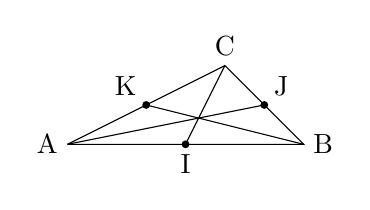
\begin{tikzpicture}
			\draw (0,0) node[left] {A} -- (3,0) node[right] {B} -- (2,1) node[above] {C} -- (0,0);
			\draw (1.5,0) node[ circle, fill, inner sep=1pt] {};
			\draw (1.5,0) node[below] {I};
			\draw (2.5,0.5) node[ circle, fill, inner sep=1pt] {};
			\draw (2.5,0.5) node[above right] {J};
			\draw (1,0.5) node[ circle, fill, inner sep=1pt] {};
			\draw (1,0.5) node[above left] {K};
			\draw (1.5,0) --  (2,1);
			\draw (2.5,0.5) --  (0,0);
			\draw (1,0.5) --  (3,0);
		\end{tikzpicture}
	\end{center}

\end{prop}

\begin{dem}{}{}
	Soit un triangle ABC, les trois bases des médianes I, J, K.
	
	Pour montrer la proposition, il suffit de montrer l'égalité suivante: 

	$$\frac{2}{3}\vec{AJ} = \vec{AB}+\frac{2}{3}\vec{BK} = \vec{AC}+\frac{2}{3}\vec{CI}$$

	Montrons la première égalité. D'après Chasles, on a $\vec{AJ} = \vec{AB} + \vec{BJ}$.

	TODO
\end{dem}

\section{Exercices}
\sectionexo{}

\end{document}


% \begin{prop}{}{}
% Lorsqu'un nombre a une écriture décimale infinie périodique c'est un nombre rationnel.
% \end{prop}

% \begin{rem}{}{}
% On dit que l'écriture est périodique lorsqu'une série de chiffre se reproduit indéfiniment.
% \end{rem}


